\documentclass[12pt]{article}

\usepackage[margin=1in, paperwidth=8.5in, paperheight=11in]{geometry}
\usepackage{amsfonts}
\usepackage{amssymb}
\usepackage{centernot}
\usepackage{amsmath}
\usepackage{pifont}
\usepackage{minted}
\usepackage{xcolor}
\usepackage{mdframed}
\usepackage{graphicx}
\usepackage{fancyhdr}
\usepackage{hyperref}

\pagestyle{fancy}
\lhead{Numerical Approximation of Eigenvalues}
\chead{}
\rhead{\thepage}
\cfoot{}

\title{
  \textbf{Numerical Approximation of Eigenvalues}\\
  \Large \textit{A Comparison of Power and Jacobi Methods}
}

\author{
  Gage Golish\\
  Department of Mathematics and Computer Science\\
  Indiana State Univeristy
}

\date{Fall 2019}

\newcommand{\codefromfile}[1]{
  \begin{mdframed}[
      backgroundcolor=black!10,
      linewidth=0pt   
  ]
  \inputminted{python}{#1}
  \end{mdframed}
}

\newcommand{\snippetfromfile}[3]{
  \begin{mdframed}[
      backgroundcolor=black!10,
      linewidth=0pt
  ]
    \begin{center}
      \dotfill\texttt{#1 (#2-#3)}\dotfill
      \inputminted[firstline=#2, lastline=#3, linenos]{python}{#1}
    \end{center}
  \end{mdframed}
}


\begin{document}

\maketitle
\thispagestyle{empty}

\pagebreak

\tableofcontents

\pagebreak

\section{Power Method}
The power method is an iterative method that numerically approximates the
largest in magnitude eigenvalue and its corresponding eigenvector of a linear
system. The only requirement is that the eigenvalues of the matrix be real.
Although the matrix does not have to also be symmetric, we test the algorithm
only on symmetric matrices for comparison purposes with the Jacobi method.

The algorithm is shown below. It was implemented as a generator function,
therefore the stopping condition is left up to the calling function. This will
be demonstrated in the results section. Each iteration takes $O(n^2)$ time due
to the matrix multiplication on line 12.
\snippetfromfile{eigen.py}{8}{16}

\section{Jacobi Method}
The Jacobi method is also an iterative method, but it approximates all
eigenvalues of the system; however, for the purposes of comparison, we will
only consider the case of the largest eigenvalue. Also the Jacobi method
requires a symmetric matrix. The functions below are subroutines of the main
Jacobi algorithm. \texttt{outer\_norm} calculates the $N(A)$ and
\texttt{outer\_argmax} finds the largest in magnitude non-diagonal entry in the
matrix. Each iteration of Jacobi costs $O(n^2)$ due to calling
\texttt{outer\_argmax} on line 22. Note that Jacobi is also implemented as a
generator and its stopping condition is left up to the calling function.
\snippetfromfile{utils.py}{6}{10}
\snippetfromfile{utils.py}{13}{17}
\snippetfromfile{eigen.py}{18}{41}

\section{Results}
In order to compare the methods, a 10x10 symmetric matrix with random values
between 0 and 20 is generated. The matrix is listed below and is referred to as
test case 3 for the purposes of the experiment. The maximum eigenvalue of the
matrix is found to be 102.85. The code for running the experiment for each
method is shown below.

\snippetfromfile{tests.py}{34}{43}
\snippetfromfile{tests.py}{44}{54}

The threshold value, $\epsilon$, is used in both iterations as the stopping
condition. Its default value is $\epsilon=0.0001$. For the power method,
$\epsilon$ is interpreted as the accuracy up to a certain number of decimal
places. For the Jacobi method, it serves as the accuracy to certain number of
decimal places for the largest in magnitude eigenvalue on the diagonal of
$A^{(m)}$. Thus the iteration will stop once the largest eigenvalue has been
approximated to the same degree of accuracy as in the power method, regardless
of how well the other eigenvalues have been approximated.

$$ A = 
\begin{bmatrix}
3.16 & 9.52 & 16.81 & 17.04 & 7.27 & 8.56 & 2.7 & 9.19 & 11.82 & 9.4 \\
9.52 & 2.74 & 12.47 & 15.97 & 4.54 & 18.59 & 3.57 & 12.65 & 15.87 & 7.27 \\
16.81 & 12.47 & 1.72 & 8.25 & 12.87 & 7.7 & 4.49 & 3.6 & 8.99 & 8.75 \\
17.04 & 15.97 & 8.25 & 4.86 & 12.4 & 6.68 & 13.69 & 10.03 & 5.3 & 10.58 \\
7.27 & 4.54 & 12.87 & 12.4 & 9.1 & 13.06 & 11.31 & 17.05 & 1.86 & 15.18 \\
8.56 & 18.59 & 7.7 & 6.68 & 13.06 & 6.11 & 13.74 & 4.83 & 5.24 & 10.14 \\
2.7 & 3.57 & 4.49 & 13.69 & 11.31 & 13.74 & 11.17 & 14.77 & 11.98 & 5.84 \\
9.19 & 12.65 & 3.6 & 10.03 & 17.05 & 4.83 & 14.77 & 18.12 & 5.32 & 11.24 \\
11.82 & 15.87 & 8.99 & 5.3 & 1.86 & 5.24 & 11.98 & 5.32 & 15.37 & 11.81 \\
9.4 & 7.27 & 8.75 & 10.58 & 15.18 & 10.14 & 5.84 & 11.24 & 11.81 & 8.48 \\
\end{bmatrix}
$$

Refer to the figure below to see the results of the experiment. As you can see,
the power method approximated the eigenvalue to within $\epsilon$ in 13
iterations, where Jacobi only took 10. The difference becomes much larger as
the required degree of accuracy is increased. In the second figure, we see that
the power method took 25 iterations where Jacobi still only took 10 when
$\epsilon=0.0000000001$.
\begin{figure}[H]
  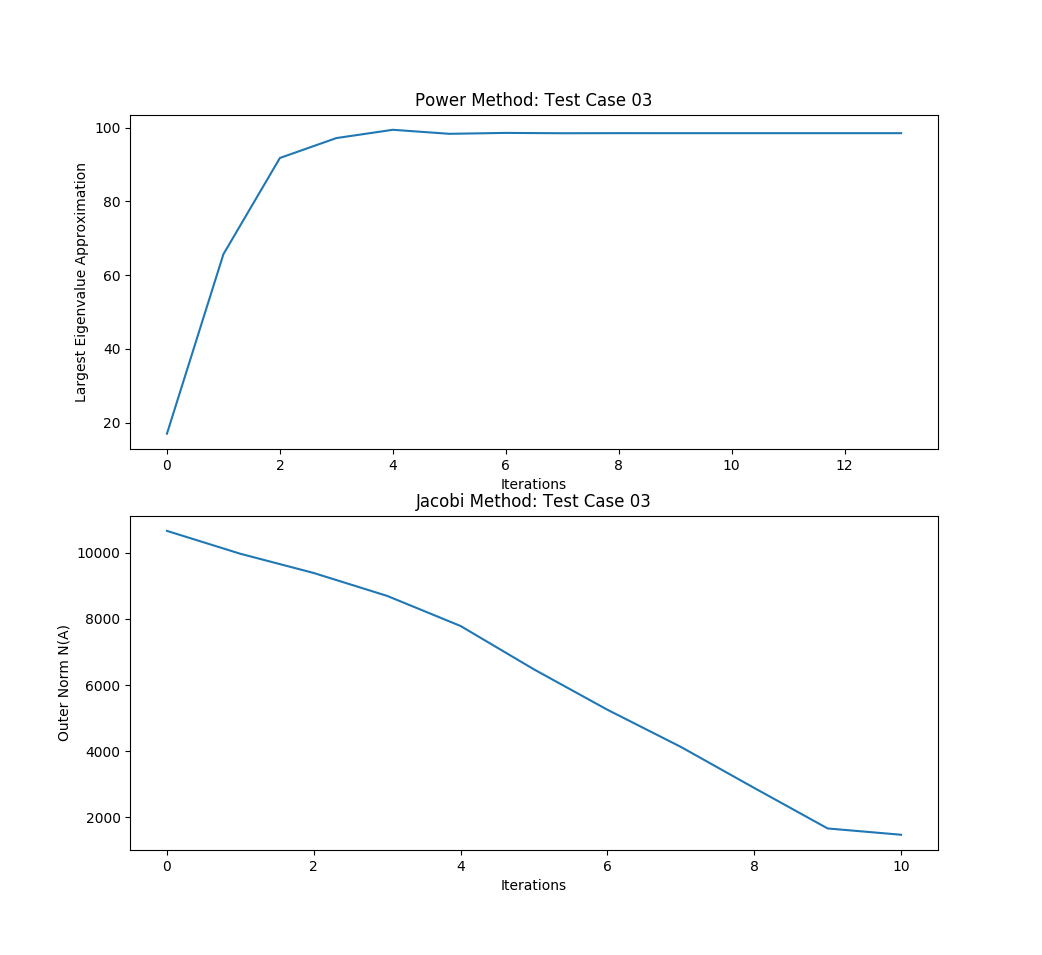
\includegraphics[width=6.5in]{figures/figure1.png}
  \caption{Plot of iterations for both Jacobi and power methods,
  $\epsilon=0.0001$.}
\centering
\end{figure}
\begin{figure}[H]
  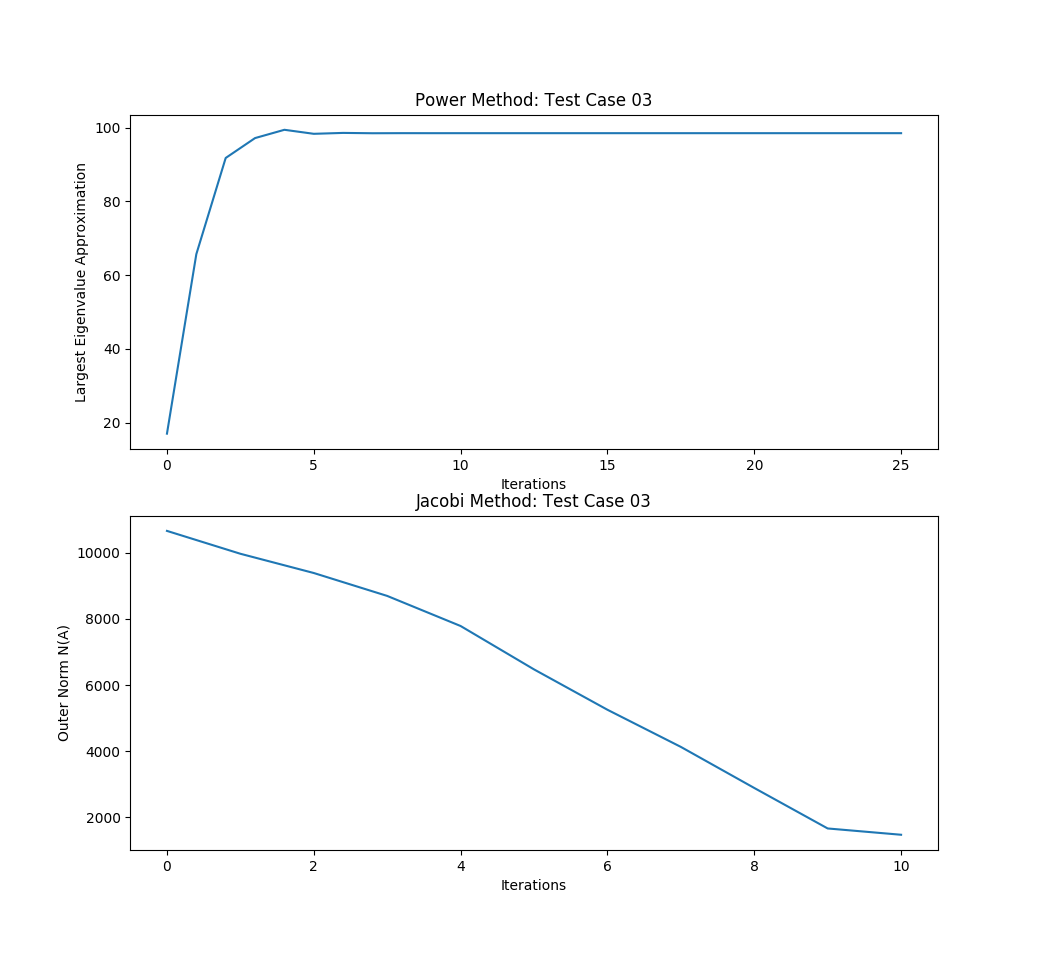
\includegraphics[width=6.5in]{figures/figure2.png}
  \caption{Plot of iterations for both Jacobi and power methods,
  $\epsilon=1\times10^{-10}$.}
\centering
\end{figure}

\end{document}
